\documentclass{config}
\usepackage[T1]{fontenc}
\usepackage[utf8]{inputenc}
\usepackage{graphicx}
\usepackage{color}
\usepackage{siunitx}
\usepackage{listings}
\usepackage{wrapfig}
\usepackage{subcaption}
\usepackage{float}
\usepackage[toc,page]{appendix} 
\usepackage{amsmath}
\usepackage{bigints}
\usepackage{colortbl}
\newcommand\x{\XSolid}

\usepackage[labelfont=sc]{caption}
\title{Aortic Clamping}
%\author{Jeanne VENTRE}

%\instlabel{}{Master 2 of Engineering in Fluid Mechanics Fundamentals and Applications, Pierre and Marie Curie University (UPMC)}

\begin{document}

\maketitle
\section{Introduction}

Lumped parameter model is the first level of modeling. They are an analogy of electrical models and are constituted of an assembly of resistances, compliances and inductances. Electrical circuits typically link tension to intensity. Lumped parameter models allow to connect the inlet flow rate to the pressure gradient between the inlet and the outlet. 

\section{Windkessel model}

In this section, we study the Windkessel model which is the most commonly used zero-dimensional (0D) parameter model to study blood flow. The windkessel model is composed of two resistances, one compliance and one inductance. In our case, this inductance will be set to zero and therefore does not appear on Fig. \ref{windkessel_schema}.

\begin{figure}[H]
\centering
\includegraphics[scale=0.3]{Figures/resistance.png}
\caption{Electrical representation of the Windkessel 0D model.}
\label{windkessel_schema}
\end{figure}

To model a vessel of lenght L,the general governing equation of a Windkessel model is the following:

\begin{equation}\label{windkessel_equation}
\left(1+ R_2 C \frac{\mathrm{d} .}{\mathrm{d}t} + I C \frac{\mathrm{d}^2 .}{\mathrm{d}t^2}\right) p(x=0) - p(x=L) =  \left( (R_1 + R_2) + R1 \left( R_2 C \frac{\mathrm{d}.}{\mathrm{d}t} + IC \frac{\mathrm{d}^2 .}{\mathrm{d}t^2}\right) + I \frac{\mathrm{d}.}{\mathrm{d}t}\right) Q(x=0).
\end{equation}

Considering that $p(x=L)$ = 0 and $I=0$, we can discretize this equation with an explicit Euler scheme that gives:

\begin{equation}\label{windkessel_euler}
p^n+ R_2 C \frac{p^{n+1} - p^n}{\Delta t} = (R_1 + R_2) Q^n + R_1 R_2 C \frac{Q^{n+1} - Q^n}{\Delta t}.
\end{equation}

In Eq. (\ref{windkessel_euler}) the unknown is $p^{n+1}$ that is the pressure at $x=0$ at time $t_{n+1}$. The flow rate $Q^n$ and $Q^{n+1}$ correpond to the inlet flow in $x=0$ that we impose. 

\section{Method}

\subsection{Input flow rate}

The inflow boundary condition $Q(x=0)$ is a flow rate thats mimics a heart pulse. The input flow rate is a half sine signal (see Fig. \ref{input_flow_rate}) described by two parameters: the amplitude $Q_0$ and the ejection time $T_{ej}$, which is a portion of heart beat $T$ fixed by the experimental data. We defined the following function: 

\begin{equation}\
f(t,\alpha) = \left\{ \begin{array}{ll}
\displaystyle \sin (\pi t/\alpha)  & ~ \text{ if }   ~ t < \alpha \\ 
\displaystyle 0    & ~ \text{ if }   ~ t > \alpha
\end{array} \right.
\end{equation}

The input flow rate is then defined as: 
\begin{equation}
Q_{input} (t) = Q_0 .  f(t/T - E(t/T), T_{ej})
\end{equation}

where $Q_0$ is the amplitude,  the function $E(t)$ is the integer-valued function, $T$ is the heart period and $T_{ej}$ is the ejection fraction. This function is represented in Fig. \ref{input_flow_rate}.

\begin{figure}[H]
\centering
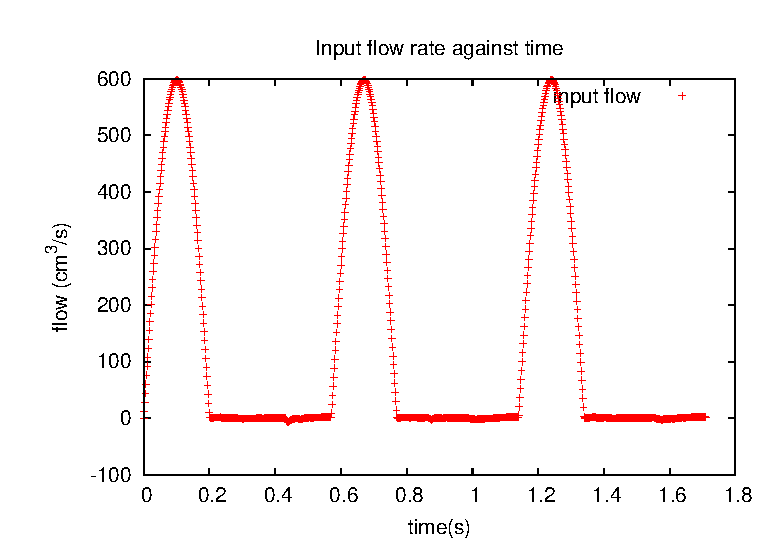
\includegraphics[scale=0.6]{Figures/input_flow.eps}
\caption{Input flow rate $Q$ as a function of time with amplitude $Q_0 =$ 350 cm$^3$/s and ejection time $T_{ej} = 40 \%$ of heart time period $T = 1$ s .}
\label{input_flow_rate}
\end{figure}

In the following, we decide not to estimate $Q_0$ the amplitude of input flow rate since it is obviously related to the value of resistance through Ohm's law ($P = R Q$). Therefore the chosen value for $Q_0$ is such that the stroke volume (i.e ventricular ejection volume over a heart beat) is comprised between 70 and 90 mL. 

\subsection{Cost function}

Now the objective is for both pre clamp and post clamp to estimate the values $R_1$, $R_2$,  $C$ along with the ejection fraction $T_{ej}$ for each patient. Therefore, we define a cost function $J$ that depends on these parameters as follows:

\begin{equation}
J(\mathrm{p}) =\left( \int_0^T (P_{exp} - P_{num}(\mathrm{p})) ^2 \mathrm{d}t \right)^{1/2}
\end{equation}

where $P_{exp}$ is the experimental pressure wave and $P_{num}$ is the solution of Eq. (\ref{windkessel_equation}) and $\mathrm{p}$ is the set of parameterss $(R_1, R_2, C,T_{ej}) $. \\ 

We use a gradient-based algorithm L-BFGS-B that allows bound type of constraints and combine it with a Basin-Hopping method to find the global extrema for each situation. \\

\section{Results}

Table \ref{param_est_tab} below sums up the results of parameter estimation on all patients for pre clamp and post clamp. We added the values of the total resistance $R_{tot} = R_1 + R_2$ and the amplitude of input flow rate $Q_0$. This last parameter is not estimated with the algorithm for obvious reasons but is adjusted so that the stroke volume $V_s$ is constant during clamping. We chose to keep the stroke volume constant because we expect that the heart has not responded yet to clamping within the period of acquisition of data. The last column corresponds to the calculated relaxation time $\tau = R_2 C$.\\

\begin{table}[H]
\begin{center}
\begin{tabular}{|>{\columncolor[gray]{0.95} \color{black}} c|c|c|c|c|c|c|c|c|c|}
\hline
\rowcolor[gray]{0.85} \textbf{Patient 6}  & $R_1$ & $R_2$ & $C$ & $T_{ej}$ &  $R_{tot}$ & $Q_0$  & $V_s$ & $\tau$\\
\hline 
Pre Clamp  & 220 & 1294 & 1.31e-3 & 32.8 & 1514 & 350 & 83.3 & 1.70  \\ 
\hline 
Post Clamp  & 287 & 1428 & 9.49e-4 & 31.6 & 1715 & 317 & 83.4 & 1.36\\ 
\hline
Pre/Post ratio & 0.77 & 0.91 & 1.38 & 1.04 & 0.88 & 1.10 & --- & 1.25\\
\hline 
\hline
\rowcolor[gray]{0.85} \textbf{Patient 7}  & $R_1$ & $R_2$ & $C$ & $T_{ej}$ &  $R_{tot}$ & $Q_0$  & $V_s$ & $\tau$\\
\hline 
Pre Clamp & 152 & 1209 & 1.18e-3 & 33.7 & 1361 & 400 & 88.4 & 1.43 \\ 
\hline 
Post Clamp  & 194 & 1214 & 1.15e-3 & 34.9 & 1408 & 380 & 88.5 & 1.40 \\ 
\hline
Pre/Post ratio & 0.78 & 0.99 & 1.03 & 0.97& 0.65 & 1.05 &  --- & 1.02  \\
\hline
\hline
\rowcolor[gray]{0.85} \textbf{Patient 9} & $R_1$ & $R_2$ & $C$ & $T_{ej}$ &  $R_{tot}$ & $Q_0$  & $V_s$ & $\tau$\\
\hline 
Pre Clamp & 122 & 1059 & 1.8e-3 & 39.6  & 1180 & 300 & 73.3 & 1.91 \\ 
\hline 
Post Clamp &  165 & 1240 & 1.4e-3 & 40.2 & 1405 & 278 & 73.3 & 1.74  \\ 
\hline
Pre/Post ratio & 0.74 & 0.85 & 1.29 & 0.99 & 0.84 & 1.08 & --- & 1.09  \\
\hline
\hline
\rowcolor[gray]{0.85} \textbf{Patient 14}  & $R_1$ & $R_2$ & $C$ & $T_{ej}$ &  $R_{tot}$ & $Q_0$  & $V_s$ & $\tau$ \\
\hline 
Pre Clamp & 110 & 698 & 2.50e-3 & 52.1 & 808 & 400 & 77 & 1.75   \\ 
\hline 
Post Clamp  & 219 & 778 & 1.91e-3 & 53.4 & 997 & 359 & 76.9 & 1.49 \\ 
\hline
Pre/Post ratio & 0.50 & 0.90 & 1.31 & 0.98 & 0.81 & 1.11 & --- & 1.17 \\
\hline 
\hline 
\textbf{Mean ratio} & 0.70 & 0.91 & 1.25 & 0.99 & 0.80 &  1.09 & --- & 1.13 \\
\hline 
\end{tabular}
\caption{Sum up of parameter estimation results of Windkessel model. Resistances $R_1$ and $R_2$ are in g.cm$^{-4}$.s$^{-1}$, compliance is in g$^{-1}$.cm$^4$.s$^{2}$, amplitude of flow rate is in cm$^3$/s, ejection fraction is in percentage of heart period, stroke volume is in cm$^3$ and $\tau$ is in s. $R_{tot}$ corresponds to the total resistance $R_1 + R_2$. }
\label{param_est_tab}
\end{center}
\end{table}

We observe that for patient 6, the ejection time decreases with clamping whereas it increases for other patients under the condition that thee stroke volume remains constant. It is probably due to the fact that patient 6 has a significant difference of heart beat before and after clamping (1.14 s before clamping vs 1.31s after clamping). However the mean change in ejection time is very small so this result is not truly relevant.  

\begin{figure}[H]
\begin{minipage}{0.48\textwidth}
\includegraphics[scale=0.5]{Figures/6preclamp.eps}
\end{minipage}
\begin{minipage}{0.48\textwidth}
\includegraphics[scale=0.5]{Figures/6postclamp.eps}
\end{minipage}

\begin{minipage}{0.48\textwidth}
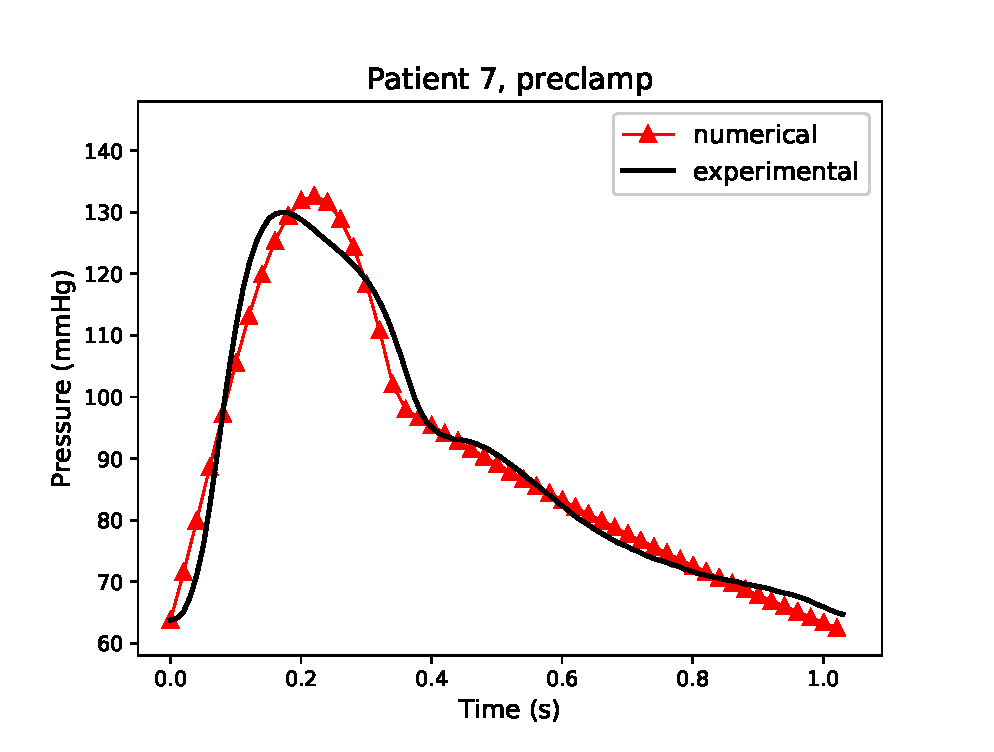
\includegraphics[scale=0.5]{Figures/7preclamp.eps}
\end{minipage}
\begin{minipage}{0.48\textwidth}
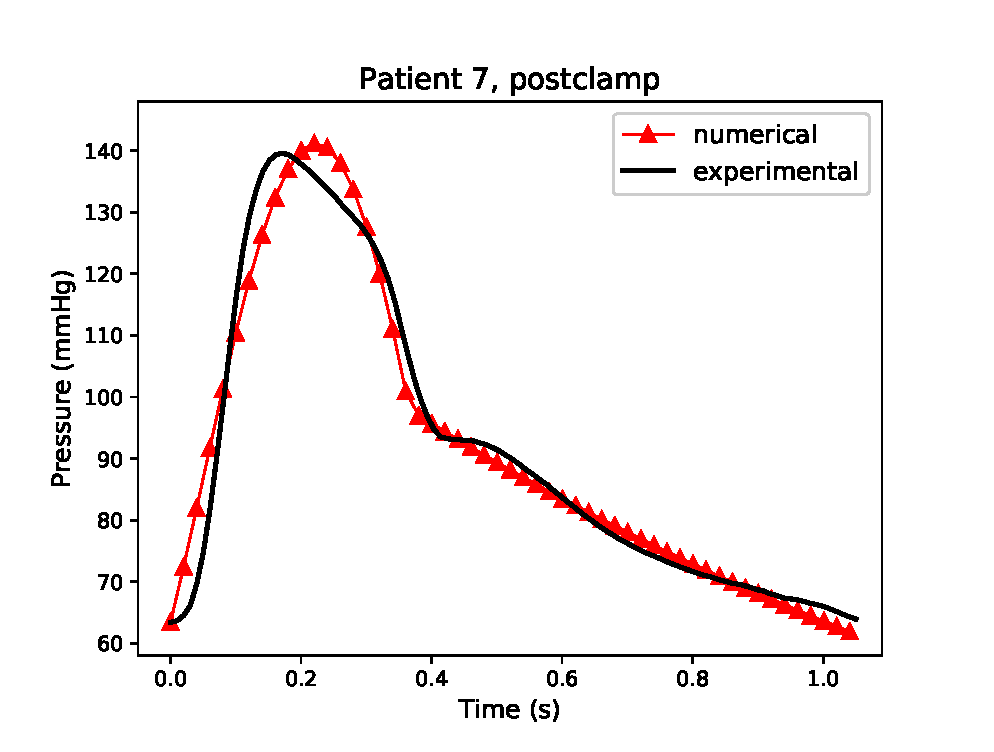
\includegraphics[scale=0.5]{Figures/7postclamp.eps}
\end{minipage}

\begin{minipage}{0.48\textwidth}
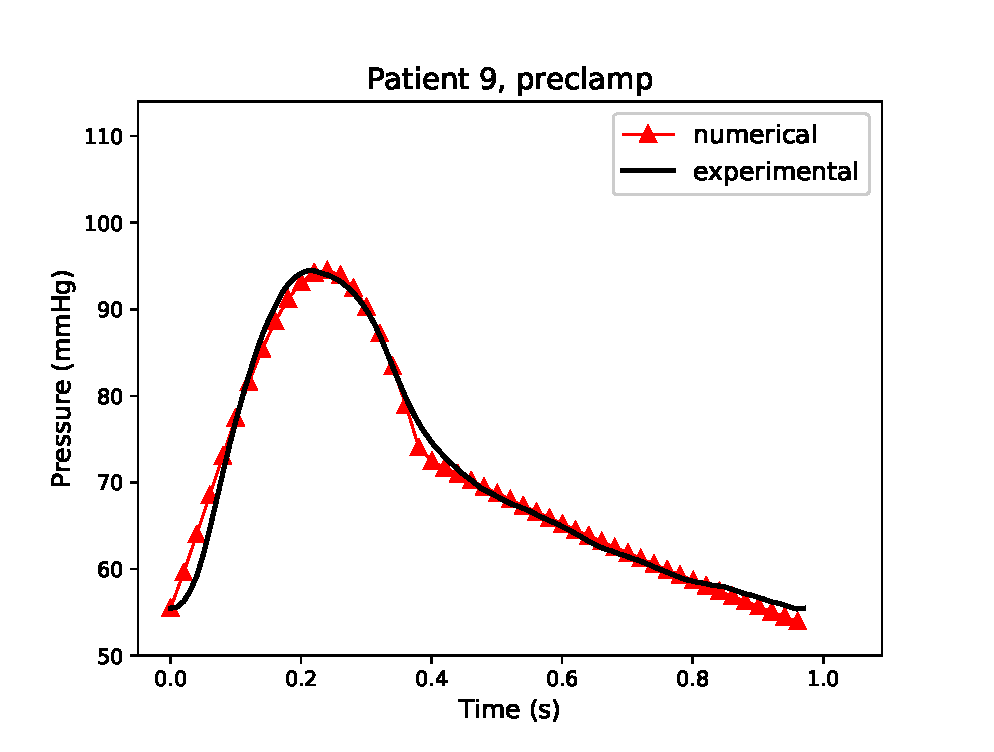
\includegraphics[scale=0.5]{Figures/9preclamp.eps}
\end{minipage}
\begin{minipage}{0.48\textwidth}
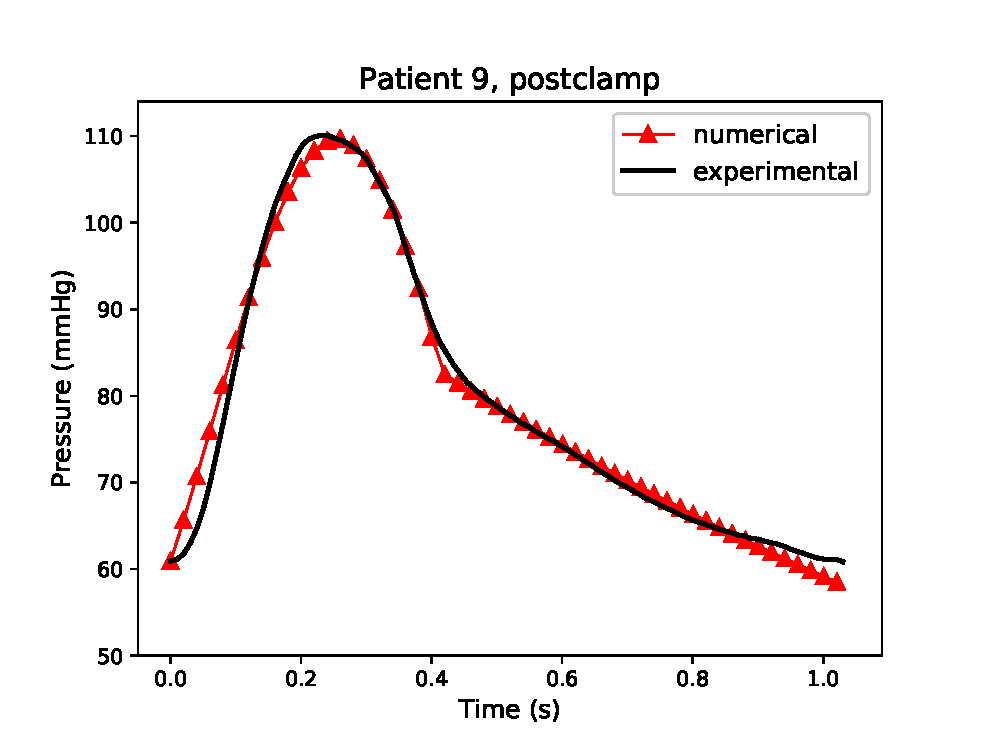
\includegraphics[scale=0.5]{Figures/9postclamp.eps}
\end{minipage}

\begin{minipage}{0.48\textwidth}
\includegraphics[scale=0.5]{Figures/14preclamp.eps}
\end{minipage}
\begin{minipage}{0.48\textwidth}
\includegraphics[scale=0.5]{Figures/14postclamp.eps}
\end{minipage}
\caption{Pressure wave signal for 4 patients undergoing aortic clamping during vascular surgery. Black lines are the experimental measurements and red corresponds to the numerical solution of Eq. \ref{windkessel_euler}}.
\label{res}
\end{figure}



%We decide to use the gradient-based method L-BFGS-B. It is a limited memory quasi-Newton code that solves large non linear optimization problems without constraints but with bounds \cite{LBFGSB}. The main idea of this method is to avoid constructing the Hessian matrix and construct instead an approximation of the inverse of the second derivative of the function to minimize by analyzing the gradient. This approximation of the derivatives allows to use Quasi-Newton's method to find the minimum in the parameter space. \\ 
%
%The algorithm is as follows, where $f(\mathbf{x})$ is the function to minimize. \\ 
%
%From $x_0$ the initial guess and a suitable approximation of the Hessian matrix $B_0$. Choose an integer $m$ that determines the number of limited memory corrections are stored. The following iterations are repeated until $x$ converges to the solution satisfying a convergence criterion:
%
%\begin{enumerate}
%\item find $\mathbf{p_k}$ solving $B_k \mathbf{p_k}  = - \nabla f(\mathbf{x_k})$ where $\mathbf{p_k}$ is the direction of the descent at step $k$. \\
%\item find the optimal time step $\alpha_k$ in the direction found from the previous step. \\
%\item update the solution: $ \mathbf{x_{k+1}} =\mathbf{x_{k}} + \alpha_k \mathbf{p_k} = \mathbf{x_k} + \mathbf{s_k} $. \\
%\item $\mathbf{y_k} =  \nabla f(\mathbf{x_{k+1}})-\nabla f(\mathbf{x_k})$. \\
%\item update the value of the Hessian matrix using the information from previous iteration: $B_{k+1} = B_k + \displaystyle \frac{\mathbf{y_k} \mathbf{y_k}^T }{\mathbf{y_k}^T \mathbf{s_k}} - \frac{B_k \mathbf{s_k} \mathbf{s_k}^T B_k}{ \mathbf{s_k}^T B_k \mathbf{s_k}}. $\\
%\end{enumerate} 
%
%Convergence can be tested by calculating the norm of the gradient $|\nabla f(\mathbf{x_k})|$. The matrix $B_0$ can be initialized with the identity matrix in which case the first iteration will be equivalent to a gradient algorithm and further steps will refine $B$. Calculating analytically the gradient of $f$ if possible will speed up the process of convergence.\\
%
%This method will only allow us to find a local minimum of $f$, depending on the initial conditions. This is why we will use a Basin Hopping algorithm. It is a stochastif algorithm that attempts to find the global minimum of a function of one of more variables. It is an iterative process and it follows these different steps: 
%
%\begin{enumerate}
%\item it creates a random perturbation of the parameters, \\
%\item it applies the method of local minimization (in our case L-BFGS-B is used),  \\
%\item it accepts or rejects the parameters found from the minimization based on the value of the functionnal. 
%\end{enumerate}

\end{document}